\documentclass{article}

\usepackage{amsmath}
\usepackage{amssymb}
\usepackage{listings}
\usepackage{color}
\usepackage{tcolorbox}
\usepackage{caption}
\usepackage{float}
\usepackage{subcaption}
\usepackage[export]{adjustbox}

\lstdefinestyle{shared}{
    belowcaptionskip=1\baselineskip,
    breaklines=true,
    xleftmargin=\parindent,
    showstringspaces=false,
    basicstyle=\fontsize{10}{6}\ttfamily,
}
\lstdefinestyle{java}{
    style=shared,
    language=Java,
    keywordstyle=\bfseries\color{green!40!black},
    commentstyle=\itshape\color{purple!40!black},
    identifierstyle=\color{blue},
    stringstyle=\color{orange},
}
\lstdefinestyle{txt}{
    style=shared,
}
\lstset{escapechar=@}

\newcounter{theo}[section]\setcounter{theo}{0}
\renewcommand{\thetheo}{\arabic{section}.\arabic{theo}}
\newenvironment{theorem}[2][]{%
\refstepcounter{theo}%
\ifstrempty{#1}%
{\mdfsetup{%
frametitle={%
\tikz[baseline=(current bounding box.east),outer sep=0pt]
\node[anchor=east,rectangle,fill=blue!20]
{\strut Theorem~\thetheo};}}
}%
{\mdfsetup{%
frametitle={%
\tikz[baseline=(current bounding box.east),outer sep=0pt]
\node[anchor=east,rectangle,fill=blue!20]
{\strut Theorem~\thetheo:~#1};}}%
}%
\mdfsetup{innertopmargin=10pt,linecolor=blue!20,%
linewidth=2pt,topline=true,%
frametitleaboveskip=\dimexpr-\ht\strutbox\relax
}
\begin{mdframed}[]\relax%
\label{#2}}{\end{mdframed}}


\newcounter{prf}[section]\setcounter{prf}{0}
\renewcommand{\theprf}{\arabic{section}.\arabic{prf}}
\newenvironment{proof}[2][]{%
\refstepcounter{prf}%
\ifstrempty{#1}%
{\mdfsetup{%
frametitle={%
\tikz[baseline=(current bounding box.east),outer sep=0pt]
\node[anchor=east,rectangle,fill=red!20]
{\strut Proof~\theprf};}}
}%
{\mdfsetup{%
frametitle={%
\tikz[baseline=(current bounding box.east),outer sep=0pt]
\node[anchor=east,rectangle,fill=red!20]
{\strut Proof~\thetheo:~#1};}}%
}%
\mdfsetup{innertopmargin=10pt,linecolor=red!20,%
linewidth=2pt,topline=true,%
frametitleaboveskip=\dimexpr-\ht\strutbox\relax
}
\begin{mdframed}[]\relax%
\label{#2}}{\end{mdframed}}


\newcounter{prob}[section]\setcounter{prob}{0}
\renewcommand{\theprob}{\arabic{section}.\arabic{prob}}
\newenvironment{problem}[2][]{%
\refstepcounter{prob}%
\ifstrempty{#1}%
{\mdfsetup{%
frametitle={%
\tikz[baseline=(current bounding box.east),outer sep=0pt]
\node[anchor=east,rectangle,fill=red!80]
{\strut Problem~\theprob};}}
}%
{\mdfsetup{%
frametitle={%
\tikz[baseline=(current bounding box.east),outer sep=0pt]
\node[anchor=east,rectangle,fill=red!80]
{\strut Problem~\theprob:~#1};}}%
}%
\mdfsetup{innertopmargin=10pt,linecolor=red!80,%
linewidth=2pt,topline=true,%
frametitleaboveskip=\dimexpr-\ht\strutbox\relax
}
\begin{mdframed}[]\relax%
\label{#2}}{\end{mdframed}}


\newcounter{exm}[section]\setcounter{exm}{0}
\renewcommand{\theexm}{\arabic{section}.\arabic{exm}}
\newenvironment{example}[2][]{%
\refstepcounter{exm}%
\ifstrempty{#1}%
{\mdfsetup{%
frametitle={%
\tikz[baseline=(current bounding box.east),outer sep=0pt]
\node[anchor=east,rectangle,fill=green!20]
{\strut Example~\theexm};}}
}%
{\mdfsetup{%
frametitle={%
\tikz[baseline=(current bounding box.east),outer sep=0pt]
\node[anchor=east,rectangle,fill=green!20]
{\strut Example~\thetheo:~#1};}}%
}%
\mdfsetup{innertopmargin=10pt,linecolor=green!20,%
linewidth=2pt,topline=true,%
frametitleaboveskip=\dimexpr-\ht\strutbox\relax
}
\begin{mdframed}[]\relax%
\label{#2}}{\end{mdframed}}


\newcounter{def}[section]\setcounter{def}{0}
\renewcommand{\thedef}{\arabic{section}.\arabic{def}}
\newenvironment{definition}[2][]{%
\refstepcounter{def}%
\ifstrempty{#1}%
{\mdfsetup{%
frametitle={%
\tikz[baseline=(current bounding box.east),outer sep=0pt]
\node[anchor=east,rectangle,fill=yellow!20]
{\strut Definition~\thedef};}}
}%
{\mdfsetup{%
frametitle={%
\tikz[baseline=(current bounding box.east),outer sep=0pt]
\node[anchor=east,rectangle,fill=yellow!20]
{\strut Definition~\thetheo:~#1};}}%
}%
\mdfsetup{innertopmargin=10pt,linecolor=yellow!20,%
linewidth=2pt,topline=true,%
frametitleaboveskip=\dimexpr-\ht\strutbox\relax
}
\begin{mdframed}[]\relax%
\label{#2}}{\end{mdframed}}

\let\cleardoublepage\clearpage

\title{DASS Assignment 3}
\date{\today}
\author{Animesh Sinha; Avani Gupta; Gaurang Tandon; }

\begin{document}
\pagenumbering{arabic}

\maketitle

\section{Introduction}

\subsection{Short overview}

\paragraph{} Hey there, welcome to our Bowling Game project! We were hired specifically \textit{not} to build a new system, but to \textbf{fix} an original implementation by some other team in terms of its \textbf{extensibility and modularity}, and implement only a few new features into it. We have toiled hard to deliver a codebase which is as extremely maintainable and flexible, and no top of that, satisfies popular laws about software engineering code metrics.
\paragraph{} We have also included all three features, namely:
\begin{itemize}
    \item Maximum multiplayer up to six players
    \item Being able to pause and play the game (and resume a paused game from memory)
    \item As well as view statistical information about the best and worst players.
\end{itemize}
It was interesting to note that our refactoring was effective enough that implementing all these features required small changes to the code at obvious locations.

\subsection{Contributions}

Effort put in: 24 hours of work-time by each member. Role of each member:
\begin{itemize}
    \item Gaurang: Complete Refactor (Specially reducing cyclomatic complexity, implementing observer pattern)
    \item Animesh: UI based refactors (from the View Classes), miscellaneous fixes
    \item Avani: Building Documentation and fixing several miscellaneous code quality errors
\end{itemize}

% this file is statistical
% will contain all final metric data

\section{Code Metrics}

\subsection{Plots of CodeMR}

\begin{figure}[H]
    \centering
    \begin{subfigure}{\textwidth}
        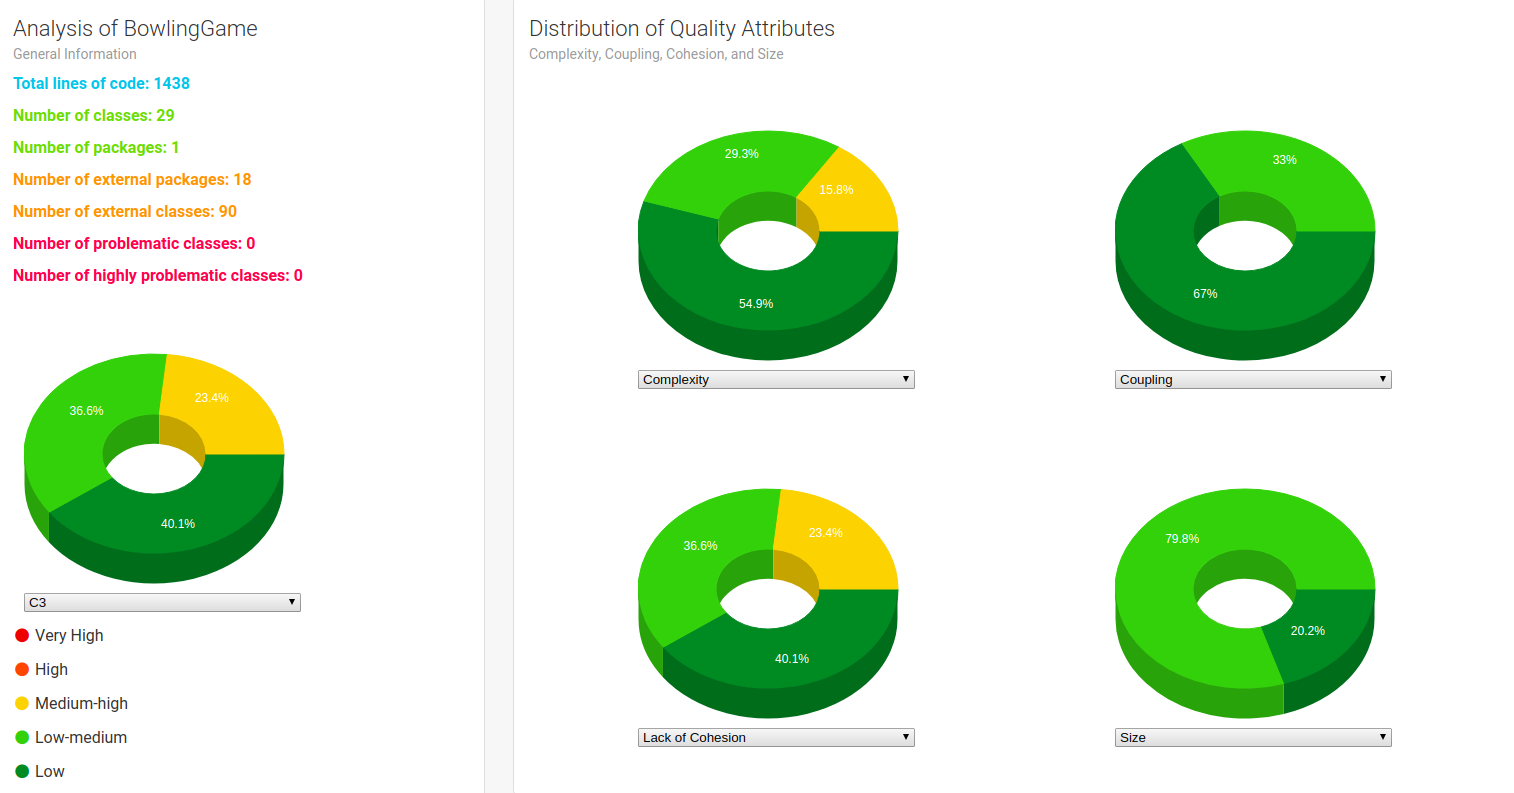
\includegraphics[width = \textwidth]{img/stats_pre.png}
        \caption{Before the Refactor}
    \end{subfigure}
    \begin{subfigure}{\textwidth}
        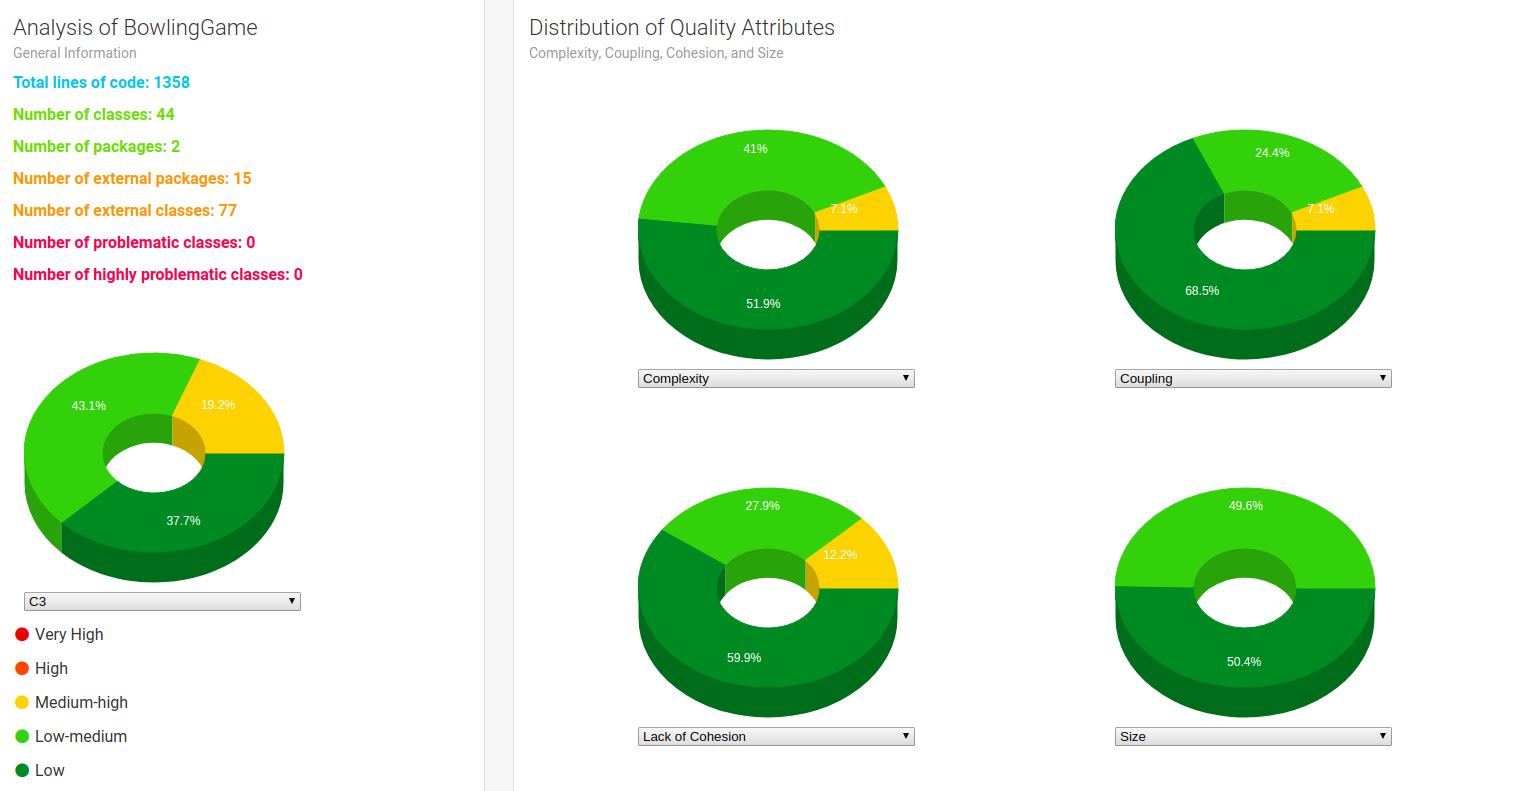
\includegraphics[width = \textwidth]{img/stats_post.png}
        \caption{After the Refactor}
    \end{subfigure}
    \caption{Code Metrics}
\end{figure}

\subsection{Metric analysis}

We investigated metrics in multiple ways: one through the CodeMR plugin for IntelliJ and the other through Metrics2 1.38 plugin for Eclipse.

\subsection{Refactoring timeline}

We present to you here the timeline of events that become the cornerstone of starting our refactoring:

\begin{itemize}

    \item Immediately, after launching metrics analyzer on the codebase, we noticed the following key components being broken: McCabe cyclomatic complexity and Nested Block Depth, with both being in Lane.java.
    \item We open Lane.java and notice it's 700 lines mammoth shape with overly complex methods. We take a guess that it's a "God class" but we're not sure.
    \item To confirm our suspicion, we look at such metrics:

          \begin{itemize}
              \item \textbf{Lack of cohesion}: it has the third highest lack of cohesion among all files.
              \item \textbf{Number of attributes}: it has the most number of attributes (18!) in a class. To be honest, 18 is a very large number and an indication that Lane.java is trying to do much.
              \item \textbf{Number of methods}: this was the killing blow. Lane.java has 17 methods, the most among all classes (the second place has only 11)
          \end{itemize}

    \item We thus concluded that Lane.java is trying to do much, and is indeed a God class.
    \item In such a system, it is ideal to start by:
          \begin{itemize}
              \item understanding all the functionality implemented in the God class
              \item marking out several sets of cohesive functionality
              \item extracting those sets out in several other classes
          \end{itemize}

    \item We then chalked out the following cohesive sets:
          \begin{itemize}
              \item Scoring functionality: \code{markScore, getScore, resetScores, isGameFinished, resetBowlerIterator}
              \item Interacting with a pinsetter: \code{getPinsetter, receivePSEvent, run}
              \item Controlling the external UI and Maintaining a observer model: \code{lanePublish, subscribe, unsubscribe, publish}
              \item Actually running the game for a party: \code{run, assignParty, isPartyAssigned}
          \end{itemize}

    \item These parts were then systematically split out into separate classes, namely, \code{ScorableParty, LaneWithPinsetter, Publisher, Lane}
    \item Once we had separate parts getting compiled, we were already ready to start ironing out complexity and redundancy issues. For quite a lot of time, we worked on these.
    \item In parallel, we also worked to ensure coupling was as low as possible.
    \item Once all was done, in the final stages, we made sure that cohesion scores were as high as possible. For classes that had lower cohesion, we grouped their properties and further increased cohesion.
    \item That was pretty much all :)
\end{itemize}

\subsection{Metric values analysis}

We have collected and analyzed the following key metrics, showing the before and after change in them as well.

\subsubsection{Lack of cohesion}

\textbf{Before:} 0.375 mean with 0.374 std.
\textbf{After:} 0.321 mean with 0.298 std.

This is the LCOM metric, calculated as a formula. Vales near 0 are good while near 1 are dangerous. This metric wasn't reduced significantly reduced, however, it was decently low before, so even the current scores are good.

\subsubsection{Coupling}
\textbf{Before:}
\textbf{After:}

\subsubsection{Nested block depth}
\textbf{Before:} 1.511 mean with 1.177 stdev
\textbf{After:} 1.423 mean with 0.659 stdev

Moreover, the largest offender Lane.java was brought down significantly. Top 3 before:

\begin{tabular}{ |c|c|c|c| }
    \hline
    \textbf{File}       & \textbf{Mean} & \textbf{Std. Dev} & \textbf{Maximum} \\
    \hline
    Lane.java & 2.176          & 2.065             & 7                \\
    Lane.java           & 2.333         & 1.374             & 5                \\
    LaneView.java       & 1.6             & 1.2             & 4                \\
    \hline
\end{tabular}

and after:

\begin{tabular}{ |c|c|c|c| }
    \hline
    \textbf{File}       & \textbf{Mean} & \textbf{Std. Dev} & \textbf{Maximum} \\
    \hline
    Lane.java           & 1.5           & 0.866             & 4                \\
    ScorableParty.java           & 1.4           & 0.611             & 3                \\
    BowlerFile.java       & 2             & 0.894             & 3                \\
    \hline
\end{tabular}

\subsubsection{Instability}

\textbf{Before:} 2.319 mean with 4.062 stdev
\textbf{After:} 1.662 mean with 1.085 stdev


\subsubsection{McCabe cyclomatic complexity}

The maximum cyclomatic complexity is down significantly. These were the top four cyclomatic complexities previously:

\begin{tabular}{ |c|c|c|c| }
    \hline
    \textbf{File}       & \textbf{Mean} & \textbf{Std. Dev} & \textbf{Maximum} \\
    \hline
    Lane.java           & 5.118         & 9.498             & 38               \\
    LaneView.java       & 5.167         & 6.543             & 19               \\
    LaneStatusView.java & 3.4           & 3.878             & 11               \\
    AddPartyView.java   & 3.5           & 3.452             & 11               \\
    \hline
\end{tabular}

and these are the top four now:

\begin{tabular}{ |c|c|c|c| }
    \hline
    \textbf{File}       & \textbf{Mean} & \textbf{Std. Dev} & \textbf{Maximum} \\
    \hline
    LaneStatusView.java & 2.75          & 2.487             & 7                \\
    Lane.java           & 1.917         & 1.656             & 7                \\
    LaneView.java       & 2             & 1.414             & 5                \\
    AddPartyView.java   & 2.625         & 1.317             & 5                \\
    \hline
\end{tabular}


\subsubsection{Attribute count}

More the attributes in a class, more likely for it to be violating the Single Responsbility Principle. As is clear from the following metrics, we have ensured that such fundamental principles are not violated.


\textbf{Before:} 4.759 mean with 5.556 stdev
\textbf{After:} 2.351 mean with 2.159 stdev

The top four before:

\begin{tabular}{ |c|c|c|c| }
    \hline
    \textbf{File}       & \textbf{Count} \\
    \hline
    Lane.java           & 18 \\
    NewPatronView.java  & 17 \\
    LaneView.java       & 15 \\
    AddPartyView.java   & 14 \\
    \hline
\end{tabular}

The top four now:

\begin{tabular}{ |c|c|c|c| }
    \hline
    \textbf{File}       & \textbf{Count} \\
    \hline
    LaneStatusView.java & 8                          \\
    LaneEvent.java           & 7                    \\
    NewPatronView.java       & 6                        \\
    AddPartyView.java   & 6                         \\
    \hline
\end{tabular}


This describes the balancing done in refactored files. Our first aim was to solely reduce the cyclomatic complexity present in different methods across files. This usually meant

\begin{itemize}
    \item understanding what the method is actually doing
    \item break it down into its core parts,
    \item extract those core parts into new methods
    \item Reuse those new methods across the codebase
\end{itemize}

Splitting up each method usually meant that large top level methods were now very easy to understand (as they only called a set of related helper methods sequentially), and the helper methods themselves had narrow work, which meant they could be reused across the codebase for different top level methods.

However, this usually meant that the cohesion in a class decreased considerably, since now there existed several methods, with each method not using all of the properties. This was now the time for us to split the class into many more classes. For example, this is the precise technique we employed with Lane.java, the behemoth monster in this codebase.

We first split it out into a LaneScorer, that was supposed to handle the entire scoring logic in the Lane. Too soon, we realized that the scoring logic per bowler is being duplicated a lot. So, we split it into a BowlerScorer, which handles scoring logic for just one bowler. BowlerScorer is now used in LaneScorer, which is used in Lane. The segregation of logic is now very clear

\begin{itemize}
    \item Scoring for one bowler: BowlerScorer
    \item Scoring for an entire lane (multiple bowlers): LaneScorer
    \item Administering facilities for an entire lane: Lane
    \item GUI for one bowler's score sheet: BowlerScoreView
    \item GUI for scores of all bowlers: LaneView
\end{itemize}

(provide more detail on more splitups)

Now, we looked at duplicated code across the codebase. One feature that really stood out was the extreme disregard for redundancy in the `XView` classes, as each of them shared a series of crucial logic duplicated. For example, the logic for centering a window, or adding a button, and more. We quickly realized this and extracted out a general set of `Widget.X` classes, whose main purposes is to provide a consistent UI throughtout the codebase. This is reused throughout the codebase, and helped us creating the UI for the newer features with minimal effort.

Since our Widget.X classes were built upon the Builder pattern, we ran into the issue of Law of Demeters...

However, now we had too many classes and had to deal with too much coupling....



\end{document}
